\subsection{Readout transfers without consistent chat amplification}
Validation selects block 21 (mean-direction AUROC 0.989). At that block, the instruct mean direction achieves HC3 test AUROC 0.992, with 0.893 and 0.885 on HAP-E GPT-4o-mini and Llama-3-8B-Instruct, respectively. The corresponding base-model results are 0.993, 0.896, and 0.869. Logistic probes further improve separability (Table~\ref{tab:readout}). These measurements support a transferable readout, but not a consistent amplification from instruction tuning. Base/instruct differences vary by generator and readout. No base-model generation intervention is tested.

\begin{table*}[t]
\centering\small
\resizebox{\textwidth}{!}{\begin{tabular}{llccc}
\toprule
Model & Readout & HC3 & HAP-E GPT-4o-mini & HAP-E Llama-3-8B-I \\
\midrule
Base & Mean difference & 0.993 [0.985, 0.999] & 0.896 [0.872, 0.921] & 0.869 [0.843, 0.897] \\
Base & Logistic & 0.999 [0.998, 1.000] & 0.896 [0.868, 0.922] & 0.915 [0.888, 0.939] \\
Instruct & Mean difference & 0.992 [0.984, 0.998] & 0.893 [0.870, 0.918] & 0.885 [0.859, 0.911] \\
Instruct & Logistic & 0.999 [0.998, 1.000] & 0.898 [0.871, 0.924] & 0.936 [0.913, 0.957] \\
\bottomrule
\end{tabular}
}
\caption{Readout AUROC at the validation-selected block 21, with paired/document bootstrap 95\% intervals. HC3 has 200 test pairs; each HAP-E comparison has 180 document pairs. Logistic probes and mean-difference vectors are fit on the same 500 HC3 training pairs.}
\label{tab:readout}
\end{table*}
\begin{figure}[t]
\centering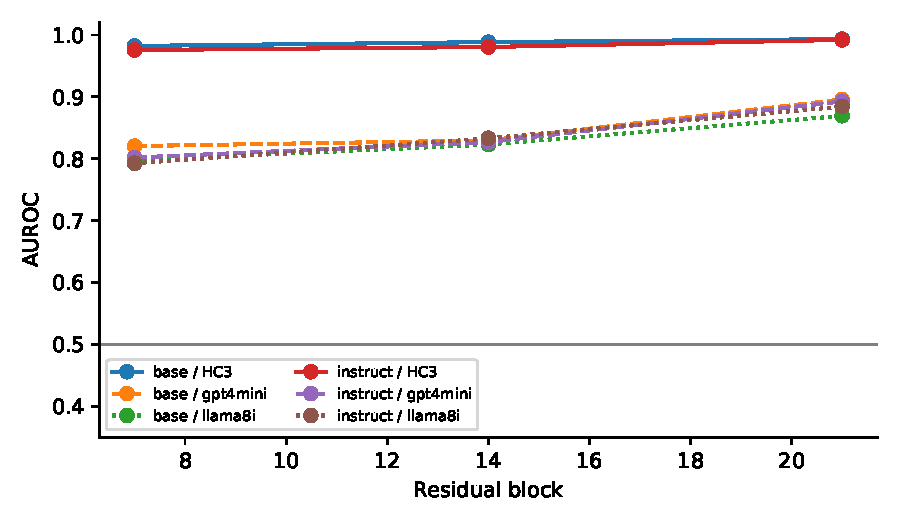
\includegraphics[width=\columnwidth]{figures/readout.pdf}
\caption{Mean-direction readout by block. Transfer remains above chance for both base and instruct models; chat tuning does not uniformly improve it.}
\label{fig:readout}
\end{figure}

Leave-one-domain-out mean-direction AUROCs range from 0.978 to 0.999 for instruct and from 0.983 to 1.000 for base (appendix). Thus the HC3 readout is not merely a classifier of the four domain labels. Matching and normalization cannot eliminate every within-domain discourse or collection artifact, however.

\subsection{A causal detector effect, with asymmetric quality costs}
In the primary sweep, quality ratings and filters use Mistral; the late audit below supplies a stricter independent assessment. Positive HC3 authorship steering raises the legacy RoBERTa score from 0.368 at baseline to 0.554 at $+1$ and 0.700 at $+2$. Paired changes are $+0.186$ [0.082, 0.292] and $+0.332$ [0.220, 0.448]. The $+1$ minus $-1$ contrast is $0.248$ [0.149, 0.355]. Because questions, decoding, and prompts are fixed, this identifies an effect of the specified residual intervention on the downstream score.

The reverse intervention is less persuasive as a humanization method. At $-1$, the score falls by 0.062, with an interval crossing zero [$-0.168$, 0.045]. At $-2$, it rises slightly rather than falling further. Adequacy drops by 0.600 points [$-0.900$, $-0.333$] and coherence by 0.333 [$-0.533$, $-0.150$]. Only 53 of 60 answers satisfy the automated quality threshold, compared with all 60 baseline answers. In contrast, positive $+1$ steering changes adequacy by 0.017 [$-0.100$, 0.117], with all answers passing. These are quality-proxy outcomes, not proof of factual equivalence.

\begin{figure*}[t]
\centering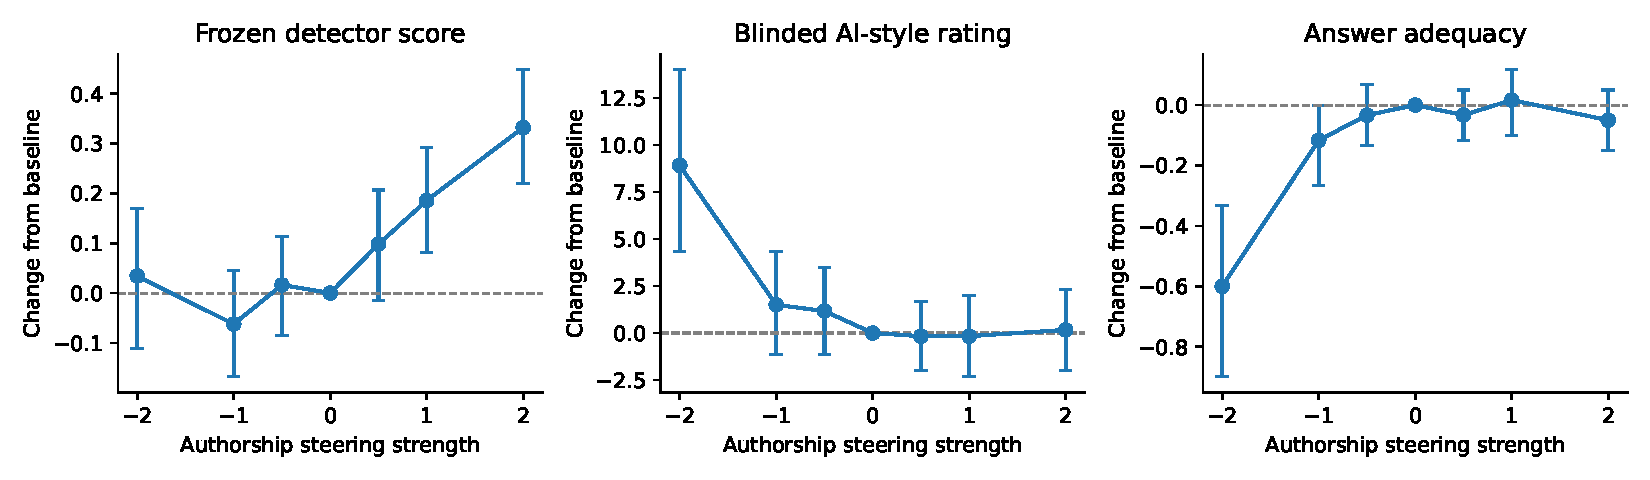
\includegraphics[width=\textwidth]{figures/dose.pdf}
\caption{Primary HC3-direction dose response, relative to the same-question baseline. Error bars are paired 95\% bootstrap intervals. The AI-style judge is unsuccessful at provenance discrimination (Table~\ref{tab:calibration}), so its near-flat response cannot validate or refute perceptual humanization. Negative extreme steering reduces rated adequacy.}
\label{fig:dose}
\end{figure*}

Centered ablation lowers RoBERTa by 0.132 [$-0.231$, $-0.031$], with mean adequacy change $-0.067$ [$-0.150$, 0.017]. The human-style prompt changes its score by $-0.062$ [$-0.162$, 0.035]. Both results are included alongside the full sweep, rather than choosing the best-performing intervention after observing outcomes. On exactly 64-token output prefixes, $+2$ retains a positive legacy-detector effect of 0.282 [0.166, 0.394], whereas the $+1$ interval crosses zero. Different eligibility sets and shorter evidence windows limit direct comparison with full answers.

\subsection{Specificity survives some, but not all, controls}
The authorship direction has cosine similarities 0.294 with formality, 0.261 with the persona proxy, 0.274 with original length, and $-0.292$ with the likelihood nuisance. Joint removal retains 89.0\% of its norm before rescaling. The orthogonalized direction still has a RoBERTa sign contrast of 0.206 [0.074, 0.334], with all 60 positive/negative pairs satisfying the quality criterion. This argues against those \emph{estimated linear nuisance axes} completely explaining the intervention.

Specificity is incomplete. The authorship sign effect exceeds the formality control by 0.362 [0.216, 0.504] and the persona proxy by 0.201 [0.033, 0.377]. It also exceeds random seed 101, but not conclusively random seed 202: the latter itself has a sign effect of 0.138 [0.027, 0.253], and the authorship-minus-random difference is 0.110 [$-0.042$, 0.272]. Two random directions are a limited sample of perturbation space. Figure~\ref{fig:controls} shows the control contrasts, and the appendix reports every condition.

\begin{figure*}[t]
\centering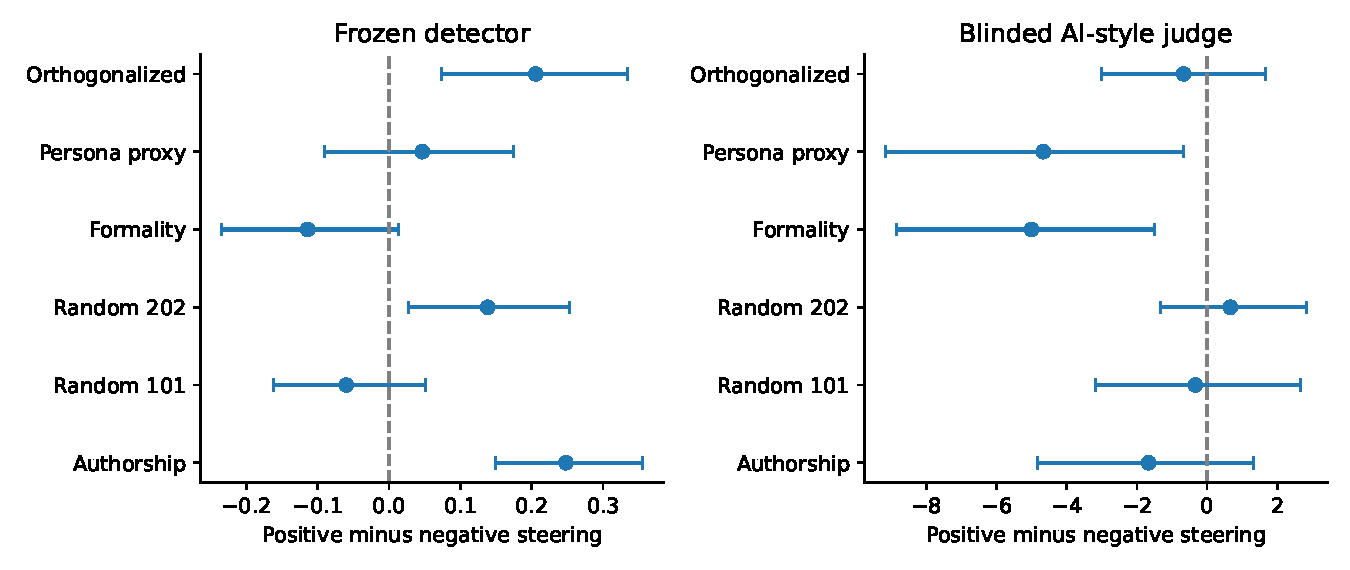
\includegraphics[width=0.93\textwidth]{figures/controls.pdf}
\caption{Positive minus negative equal-norm interventions at magnitude 1. The legacy detector responds to the authorship and nuisance-orthogonalized directions, but also to one random direction. The blinded style judge is not a reliable authorship detector on the audit sets.}
\label{fig:controls}
\end{figure*}

\subsection{Evaluator validity changes the interpretation}
The blinded judge fails our authorship-discrimination audit: its AI-style rating has AUROC 0.343 on HC3 and 0.434 on HAP-E, while assigning higher mean AI-style scores to human excerpts. We retain these ratings without reversing their sign, but do not use them as independent corroboration of an authorship effect. This audit does not supply ground-truth \emph{perceived} style labels; it shows that the chosen operational measure does not track known provenance in our samples.

We therefore added a separately labeled exploratory measure: the public Desklib DeBERTa-v3-large detector~\cite{desklib}. Its documented masked-mean-pooling sigmoid head was loaded with a strict weight-key check, without fitting or threshold tuning. On the same audit texts it achieves AUROC 0.992 on HC3 and 0.987 on HAP-E, compared with 0.933 and 0.658 for the historical RoBERTa detector (Table~\ref{tab:calibration}). Detector independence here means separate weights, architecture, and inference from the intervention model; unknown overlap in pretraining or detector training cannot be ruled out.

\begin{table}[t]
\centering\scriptsize\begin{tabular}{llrc}
\toprule
Dataset & Measure & Texts & AUROC [95\% CI] \\
\midrule
HAPE & RoBERTa & 90 & 0.658 [0.544, 0.761] \\
HAPE & Mistral judge & 90 & 0.434 [0.319, 0.553] \\
HC3 & RoBERTa & 160 & 0.933 [0.890, 0.971] \\
HC3 & Mistral judge & 160 & 0.343 [0.280, 0.406] \\
HC3 & Desklib & 160 & 0.992 [0.984, 0.998] \\
HAPE & Desklib & 90 & 0.987 [0.962, 1.000] \\
HC3 & Claude (late) & 160 & 0.856 [0.804, 0.903] \\
HAPE & Claude (late) & 90 & 0.849 [0.788, 0.906] \\
\bottomrule
\end{tabular}

\caption{Independent-measure audit on held-out natural texts. HC3 has 80 human/machine pairs; HAP-E has 30 document triplets. Intervals resample pairs/documents. Desklib was an exploratory addition.}
\label{tab:calibration}
\end{table}

Desklib scores are near ceiling on baseline generations (mean 0.990). At $-1$, the mean decreases by 0.024 [$-0.049$, $-0.004$]; the $+1$ minus $-1$ contrast is 0.028 [0.006, 0.056]. The orthogonalized sign contrast is likewise positive, 0.024 [0.008, 0.047]. Nevertheless, 58 of 60 $-1$ answers and all 60 baseline answers remain above the detector's conventional 0.5 cutoff. At $-2$, 59 remain above it. Shifting a continuous detection score is not equivalent to successful evasion.

Because sigmoid saturation obscures score movement, we additionally retained pre-sigmoid logits as an explicitly post-inspection diagnostic. The HC3 direction's $+1$ minus $-1$ logit contrast is 2.060 [1.410, 2.731], compared with 1.073 for formality, 0.105 for the persona proxy, and 0.097 and $-0.078$ for the two random directions. Its contrast exceeds formality by 0.987 [0.090, 1.897], and both random controls by intervals excluding zero. The orthogonalized logit contrast remains 1.840 [1.222, 2.483]. These exploratory results support a detection-related component beyond the fitted nuisance span, but depend on one added detector and cannot establish a universal perception axis.

The $-1$ Desklib logit shift remains negative on the 59 quality-qualified pairs ($-1.244$), and on fixed 64-token prefixes ($-1.051$ [$-1.800$, $-0.247$]). These checks reduce, but do not remove, concerns about length and gross quality. Figure~\ref{fig:modern} makes the sigmoid ceiling visible.

\begin{figure*}[t]
\centering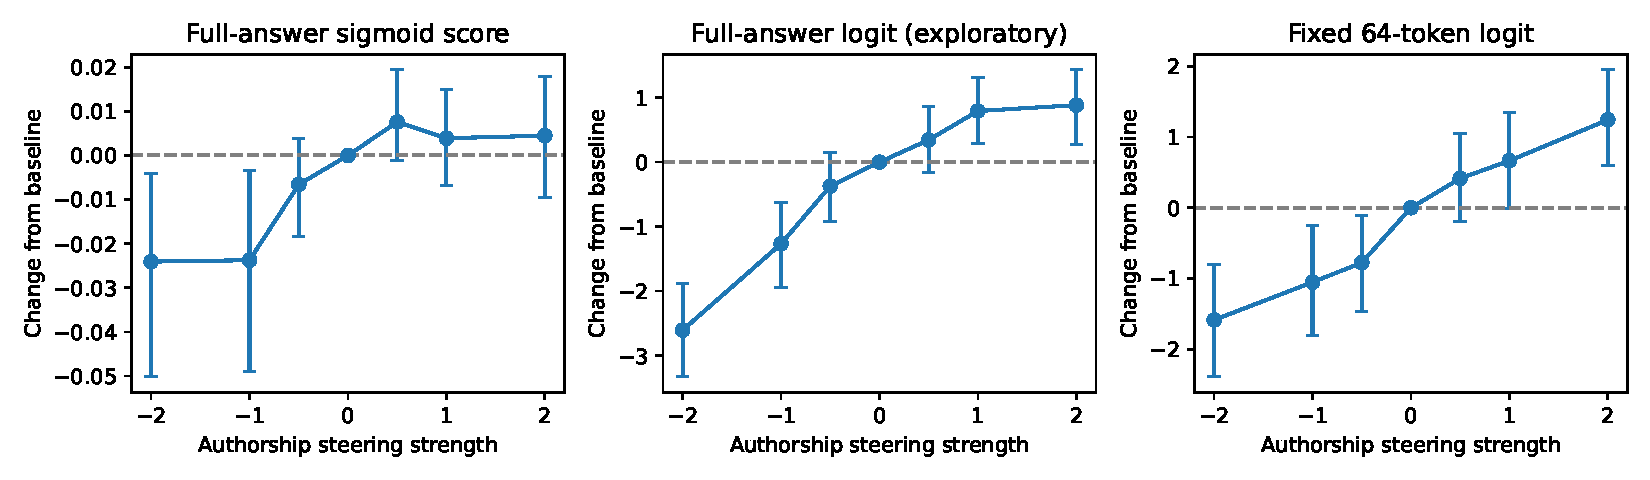
\includegraphics[width=\textwidth]{figures/modern_dose.pdf}
\caption{Exploratory Desklib outcomes. Sigmoid scores are near ceiling, so logit changes are more visible than probability-scale changes. Fixed-prefix eligibility is treatment-dependent. Logit analysis was added after inspecting saturation and is not a prespecified primary endpoint.}
\label{fig:modern}
\end{figure*}

We separately stress-tested the quality rubric on 20 baseline answers and 60 constructed corruptions, with unchanged blinded prompts. Mean coherence falls from 4.40 to 2.60 under word shuffling and to 1.60 under repetition; adequacy falls from 4.75 to 1.00 when an unrelated answer is substituted. Thus the rubric detects clear failures, even though its AI-style score does not track provenance. This audit validates sensitivity to gross corruption, not factual accuracy or subtle semantic preservation.


\subsection{Cross-corpus causal replication}
An exploratory replication fits a second mean direction on 180 additional HAP-E documents, disjoint from transfer-evaluation documents, with both machine generators contributing equally. We retain the HC3-selected block and match the HC3 vector norm. This vector has cosine 0.589 with the HC3 vector; its held-out AUROCs are 0.952 on HC3, 0.984 on HAP-E GPT-4o-mini, and 0.941 on HAP-E Llama. It therefore provides a plausible cross-corpus readout, not simply an arbitrary control.

Its 120 additional interventions reveal evaluator dependence. Positive HAP-E steering \emph{reduces} the historical RoBERTa score by 0.132 [$-0.231$, $-0.038$], whereas negative steering increases it by 0.137 [0.005, 0.271]. This reverses the expected sign despite positive geometric alignment. Desklib instead responds in the expected direction: the positive-minus-negative sigmoid contrast is 0.039 [0.009, 0.079], with logit contrast 2.712 [2.103, 3.321]. All 60 answers under either sign pass the coarse quality threshold. The same intervention can therefore increase one independently trained detector's notion of machine text and decrease another's.

Together, the HC3 and HAP-E experiments support a steerable, detection-related writing component. They do not identify an evaluator-invariant ``AI-ness'' variable. Table~\ref{tab:modernall} reports the exploratory detector results for every direction, including the transfer experiment, rather than only favorable comparisons.


\subsection{Late external style and quality audit}
\label{sec:claude}
After the UTC-day quota reset restored API access, we evaluated all fixed outputs with the originally planned Claude Haiku 4.5 rubric. This late audit followed inspection of the local results; it did not change any direction, strength, prompt, or generated answer. It contributes 1,570 additional evaluations: 1,260 intervention answers, 250 natural audit excerpts, and 60 quality corruptions. Complete raw responses are retained, including explanatory text when the service returned more than the requested JSON.

Unlike Mistral, Claude's AI-style ratings distinguish known provenance on both audits: HC3 AUROC 0.856 [0.804, 0.903] and HAP-E 0.849 [0.788, 0.906]. Its $+1$ minus $-1$ authorship-style contrast is 5.67 [2.90, 8.93] points. This supplies a second kind of evidence that the HC3 direction affects AI-like wording, beyond classifier scores. It remains an LLM judgment rather than a human perceptual experiment.

The nuisance comparison is less favorable to a distinct style axis. The formality control has a style contrast of 8.83 [5.58, 12.43], and the authorship contrast does not exceed it (difference $-3.17$ [$-7.57$, 1.23]). Orthogonalization reduces the style contrast to 1.40 [0.00, 3.20], a reduction of 4.27 [1.90, 6.98] relative to the original direction. In contrast, its trained-detector effects remain substantial. Thus detector movement after nuisance removal is stronger evidence for detection-related features than for a distinct AI-style control. The HAP-E direction has a smaller positive Claude style contrast of 2.50 [1.33, 3.67], agreeing with Desklib rather than the reversed RoBERTa response.

\begin{figure*}[t]
\centering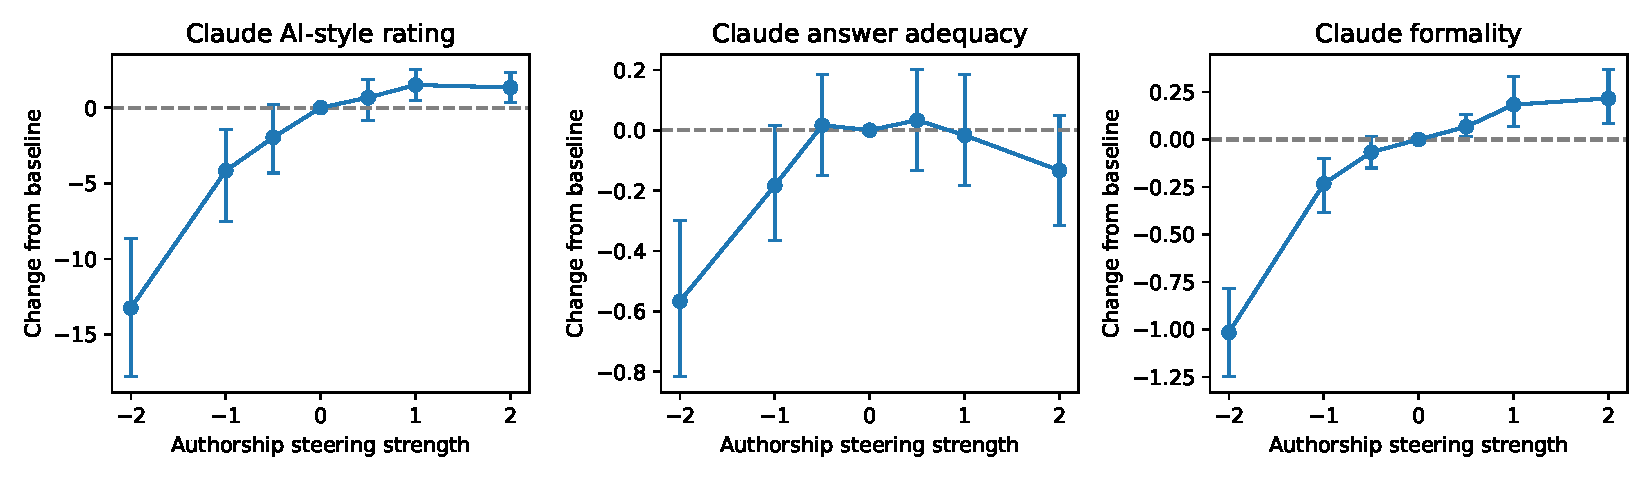
\includegraphics[width=\textwidth]{figures/claude_dose.pdf}
\caption{Late blinded Claude audit of unchanged generations. Negative authorship steering reduces rated AI-like style, but the strongest intervention also reduces answer adequacy and formality. These results were obtained after the initial local study, using its original rubric.}
\label{fig:claude}
\end{figure*}

Most importantly, Claude is substantially stricter about quality. Baseline mean adequacy is 3.10, versus Mistral's 4.78; only 23 of 60 baseline answers pass the joint threshold, versus all 60 under Mistral. At $-2$, AI style falls by 13.25 [$-17.80$, $-8.63$] points, but adequacy falls by 0.567 [$-0.817$, $-0.300$] and coherence by 0.750. At $-1$, AI style falls by 4.17 [$-7.50$, $-1.47$], with adequacy change $-0.183$ [$-0.367$, 0.017]. Only 16 baseline/$-1$ pairs satisfy Claude's quality threshold; their style change is $-1.69$ [$-7.56$, 1.88]. This small, selected subset cannot establish quality-preserving humanization.

Claude also detects known corruption: on the 20-answer quality audit, shuffling reduces coherence from 4.45 to 1.15, and unrelated answers reduce adequacy from 3.20 to 1.00. Agreement on gross corruption therefore does not imply agreement on the adequacy of plausible natural answers. The late audit materially weakens claims based on the original quality filter. All Claude condition means, changes, and quality-qualified effects are reported in Table~\ref{tab:claudeall}.

